\subsection{NMOS threshold}\label{nmos_dimensioning}
First we take a look at the worst case of 4 stacked NMOS transistors, which is the highest stacking amount which will be possible in technologies relying on this process.

%%  ************    LibreSilicon's StdCellLibrary   *******************
%%
%%  Organisation:   Chipforge
%%                  Germany / European Union
%%
%%  Profile:        Chipforge focus on fine System-on-Chip Cores in
%%                  Verilog HDL Code which are easy understandable and
%%                  adjustable. For further information see
%%                          www.chipforge.org
%%                  there are projects from small cores up to PCBs, too.
%%
%%  File:           StdCellLib/Documents/LaTeX/schematic_AND4.tex
%%
%%  Purpose:        Schematic File for AND4
%%
%%  ************    LaTeX with circdia.sty package      ***************
%%
%%  ///////////////////////////////////////////////////////////////////
%%
%%  Copyright (c) 2018 by chipforge <hsank@nospam.chipforge.org>
%%  All rights reserved.
%%
%%      This Standard Cell Library is licensed under the Libre Silicon
%%      public license; you can redistribute it and/or modify it under
%%      the terms of the Libre Silicon public license as published by
%%      the Libre Silicon alliance, either version 1 of the License, or
%%      (at your option) any later version.
%%
%%      This design is distributed in the hope that it will be useful,
%%      but WITHOUT ANY WARRANTY; without even the implied warranty of
%%      MERCHANTABILITY or FITNESS FOR A PARTICULAR PURPOSE.
%%      See the Libre Silicon Public License for more details.
%%
%%  ///////////////////////////////////////////////////////////////////
    \begin{figure}[H]
	\centering
            \begin{circuitdiagram}{50}{33}
            \pin{2}{2.5}{L}{A}  % pin A, n-channel below
            \pin{2}{8.5}{L}{B}  % pin B, n-channel middle
            \pin{2}{14.5}{L}{C} % pin C, n-channel middle
            \pin{2}{20.5}{L}{D} % pin D, n-channel above
            \pin{2}{29.5}{L}{A} % pin A, p-channel left
            \pin{14}{29.5}{L}{B} % pin B, p-channel middle
            \pin{26}{29.5}{L}{C} % pin C, p-channel middle
            \pin{38}{29.5}{L}{D} % pin D, p-channel right
            \trans{nenh*}{6}{4}{R}{}{}  % nmos below
            \trans{nenh*}{6}{10}{R}{}{} % nmos middle
            \trans{nenh*}{6}{16}{R}{}{} % nmos middle
            \trans{nenh*}{6}{22}{R}{}{} % nmos above
            \trans{nenh*}{54}{22}{R}{}{} % nmos inverter
            \trans{penh*}{6}{28}{R}{}{} % pmos left
            \trans{penh*}{18}{28}{R}{}{} % pmos middle
            \trans{penh*}{30}{28}{R}{}{} % pmos middle
            \trans{penh*}{42}{28}{R}{}{} % pmos right
            \trans{penh*}{54}{28}{R}{}{} % pmos inverter
            \wire{8}{6}{8}{8}     % wire between nmos
            \ground{8}{0.5}{D}  % ground below nmos
            \ground{56}{18.5}{D}  % ground below inverter
            \power{8}{31.5}{U}{}  % power above left pmos
            \power{20}{31.5}{U}{}  % power above middle pmos
            \power{32}{31.5}{U}{}  % power above middle pmos
            \power{44}{31.5}{U}{}  % power above right pmos
            \power{56}{31.5}{U}{}  % power above inverter
            \wire{8}{12}{8}{14}     % wire between nmos
            \wire{8}{18}{8}{20}     % wire between nmos and pmos
            \wire{20}{25}{20}{26}
            \wire{32}{25}{32}{26}
            \wire{44}{25}{44}{26}
            \wire{8}{25}{51}{25}    % wire before inverter gate
            \junct{8}{25}
            \junct{20}{25}
            \junct{32}{25}
            \junct{44}{25}
            \junct{56}{25}
            \wire{51}{29.5}{51}{20.5}   % wire at inverter gates
            \junct{51}{25}
            \wire{56}{25}{58}{25}    % wire before pin Z
            \pin{59}{25}{R}{Z}  % pin Z
            \end{circuitdiagram}
            \caption{AND4 gate}
    \end{figure}
As shown in  \autoref{TTL_logic_levels} our acceptable voltages for our CMOS "ON" state range from 2V to VDD (which typically is around $5V\pm0.25V$)

\begin{equation}
V_{on} \geq 2V
\end{equation}

Because there are four transistors dividing the voltage by being in series, the power supply voltage is being divided by the amount of transistors in series.
In order to match the threshold voltages of all of the transistors, which is needed for a working digital logic, the following equation need to be satisfied

\begin{equation}
V_{on} > 4 \cdot V_{Tn}
\end{equation}

Lets assume the worst case with

\begin{equation}
V_{on} = 2V
\end{equation}

Which leads to the required worst case threshold tolerance value

\begin{equation}
4 \cdot V_{Tn} < 2V
\Rightarrow
V_{Tn} < 500mV
\end{equation}
 
With the values derived from \autoref{gate_dimensioning} and a surface concentration for our P-well of $10^{22}\frac{1}{m^3}$ we are already set because $\approx 0.39V$ are already better than we need.

We target a concentration of $N_p = 10^{16}\frac{1}{cm^3}=10^{22}\frac{1}{m^3}$.

The depletion zone thickness at its peak will be $W_{dmax} \approx 2.73 \cdot 10^{-7} m = 273 nm$

With an implantation (or constant source diffusion step), we can now set a range/energy and dosage in order to cover the depletion zone area.

For getting the energy and dose we look at \autoref{graphics_range_and_straggle} or use the web tool linked in the implant chapter.

The depth of the p-well $\approx 2 \mu m$ comes mainly from the need to fulfill the condition from \autoref{physics_drive_in}

\begin{equation}
x_e = 2 \cdot \sqrt{D_e \cdot t_e} \gg 2 \cdot \sqrt{D_v \cdot t_v} = x_v
\end{equation}

\newpage

We already got the background ($N_B \approx 7 \cdot 10^{14} \frac{1}{cm^3}=7 \cdot 10^{20} \frac{1}{m^3}$) concentration from the specs of the basis substrate.

\begin{equation}
N_p - N_B = 10^{22}\frac{1}{m^3} - 7 \cdot 10^{20} \frac{1}{m^3} = 9.3 \cdot 10^{21} \frac{1}{m^3}
\end{equation}

We use a drive in temperature of $1150 \degree C$ which is  $T = 1423.15 \degree K$ in Kelvin which gives us the diffusion coefficient $D=9.1 \cdot 10^{-17}  \frac{m^2}{s}$

Now using
\begin{equation}
N(x,t)
=
\frac{Q}{\sqrt{\pi\cdot D \cdot t}} \cdot \exp\left(\frac{-x^2}{4 \cdot D \cdot t}\right)
\end{equation}

We set the conditions and get the required diffusion time as well as the initial dosage in one shot:
\begin{equation}
N(0,t)
=
\frac{Q}{\sqrt{\pi\cdot D \cdot t}}
=
N_p-N_B
=
7 \cdot 10^{20} \frac{1}{m^3}
\end{equation}
\begin{equation}
x
=
2 \cdot \sqrt{D \cdot t \cdot\ln\left(\frac{N_T}{N_B}\right)}
=
2 \mu m
=
2 \cdot 10^{-6} m
\end{equation}
\begin{equation}
\Rightarrow
t \approx 4259s \approx \underline{70 min}
\end{equation}
\begin{equation}
\Rightarrow
Q
=
7 \cdot 10^{20} \frac{1}{m^3} \cdot \sqrt{\pi\cdot D \cdot t}
\approx
\underline{1.02 \cdot 10^{16} \frac{1}{m^2}}
\end{equation}

If we plot the functions from our calculation we can yield the below graphics\footnote{see simulation/diffusion\_pwell.wxmx}

\begin{figure}[H]
	\centering
	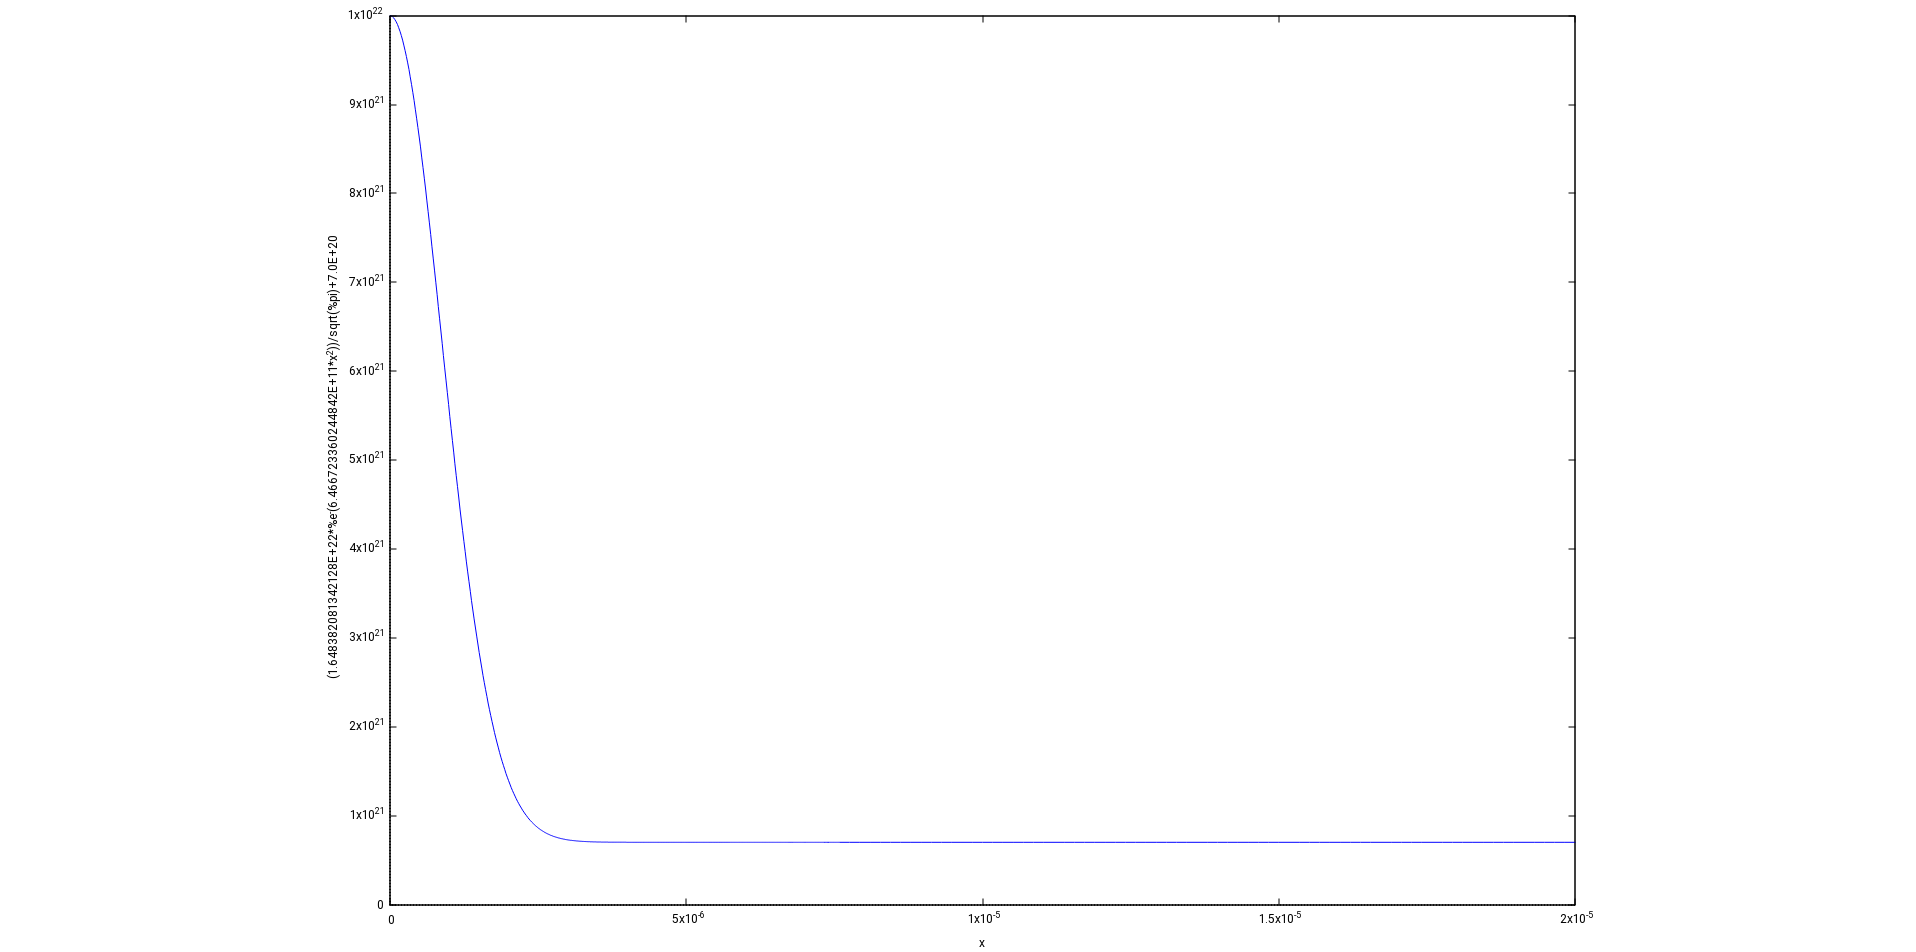
\includegraphics[width=0.75\textwidth]{p-well-diffusion.png}
	\caption{Dopant concentration after around 70 minutes}
	\label{pwell_drive_in_outcome}
\end{figure}

In \autoref{pwell_drive_in_outcome} we can see that after roughly an hour we already have the desired even gradient and deep penetration of dopants, which will give us a low $R_{DS}$.